\section{Web app}

\subsection{Introduzione e scopo del prodotto}
L'applicazione web è sviluppata per il solo utente amministratore.

In generale offre all'utente le seguenti funzionalità:
\begin{itemize}
	\item \textbf{Login:} L'utente ha la possibilità di autenticarsi inserendo il proprio username e password; \\
	\item \textbf{Logout:} L'utente ha la possibilità di deautenticarsi premendo sul bottone "Logout" del menù principale in alto a destra. \\
\end{itemize}
Per quanto riguarda le stanze, permette all'amministratore di:
\begin{itemize}
	\item \textbf{Aggiungere una stanza}: l'amministratore ha la possibilità di aggiungere una nuova stanza premendo sul bottone "Add Room"; \\
	\item \textbf{Ricercare una determinata postazione}: l'amministratore ha la possibilità di ricercare una postazione inserendo determinati parametri premendo sul bottone "Search Workstation"; \\
	\item \textbf{Modificare una stanza}: l'amministratore ha la possibilità di modificare le caratteristiche di una stanza premendo sul bottone "Edit Room"; \\
	\item \textbf{Rimuovere una stanza}: l'amministratore ha la possibilità di rimuovere una stanza premendo sul bottone "Remove Room"; \\
	\item \textbf{Aggiungere una postazione all'interno di una stanza}: l'amministratore ha la possibilità di aggiungere una postazione all'interno di una stanza premendo sul bottone "Add Workstation"; \\
	\item \textbf{Rimuovere una postazione all'interno di una stanza}: l'amministratore ha la possibilità di eliminare una postazione all'interno di una stanza premendo sul bottone dove è raffigurato un cestino; \\
	\item \textbf{Modificare una postazione all'interno di una stanza}:  l'amministratore ha la possibilità di modificare le caratteristiche di una postazione all'interno di una stanza premendo sul bottone dove è raffigurata una "E". \\
\end{itemize}
Per quanto riguarda le credenziali, permette all'amministratore di:
\begin{itemize}
	\item \textbf{Aggiungere una credenziale}: l'amministratore ha la possibilità di aggiungere una credenziale premendo sul bottone "Crea credenziale"; \\
	\item \textbf{Eliminare una credenziale}: l'amministratore ha la possibilità di eliminare una credenziale premendo sul bottone dove è raffigurato un cestino; \\
	\item \textbf{Modificare una credenziale}:  l'amministratore ha la possibilità di modificare le caratteristiche di una credenziale premendo sul bottone dove è raffigurata una "M". \\
\end{itemize}

\subsection{Requisiti e installazione}
La web app viene eseguita sul browser, non necessita di installazione e ha come unico requisito una connessione ad internet.

\subsection{Utilizzo}
\subsubsection{Login}
\begin{figure}[H]
	\centering
	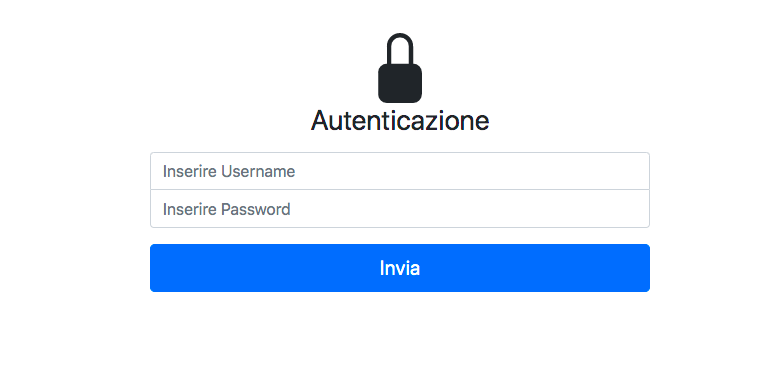
\includegraphics[width=15cm]{res/images/login.jpg}
	\caption{Login}
\end{figure}
L'amministratore può autenticarsi inserendo il proprio username e la password. L’username è da inserire nel primo campo di testo, la password nel secondo. Dopo l’inserimento dei dati può cliccare sul pulsante 'Invia' per effettuare l'autenticazione.

\subsubsection{Visualizzazione errore di autenticazione}
\begin{figure}[H]
	\centering
	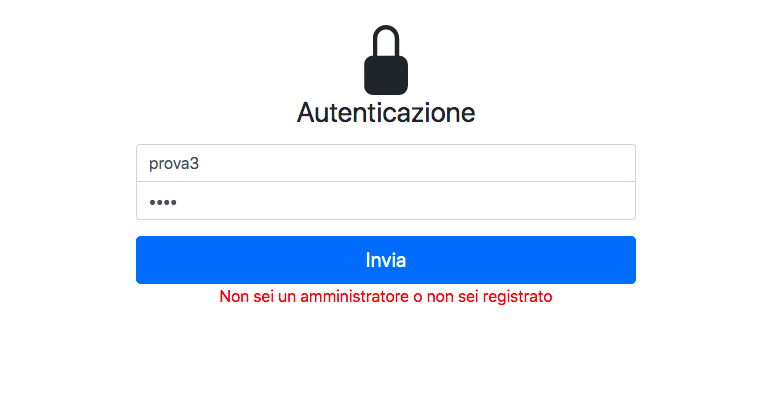
\includegraphics[width=15cm]{res/images/error.png}
	\caption{Visualizzazione errore}
\end{figure}
Se le credenziali inserite risultano errate, l’applicazione mostra un errore avvisando la persona che o non è un amministratore o ancora non è registrata.

\subsubsection{Visualizzazione errore di disabilitazione}
\begin{figure}[H]
	\centering
	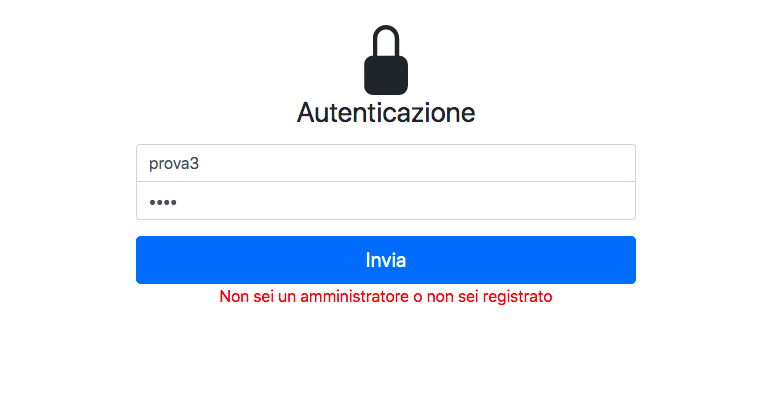
\includegraphics[width=15cm]{res/images/error.png}
	\caption{Visualizzazione errore}
\end{figure}
Se le credenziali inserite risultano disabilitate, l’applicazione mostra un errore avvisando che le credenziali inserite risultano disabilitate.
Il messaggio che viene dato all'utente è generico per evitare falle di sicurezza, perchè in qualche modo le credenziali sono ancora presenti all'interno del sistema.
\subsubsection{Logout}
\begin{figure}[H]
	\centering
	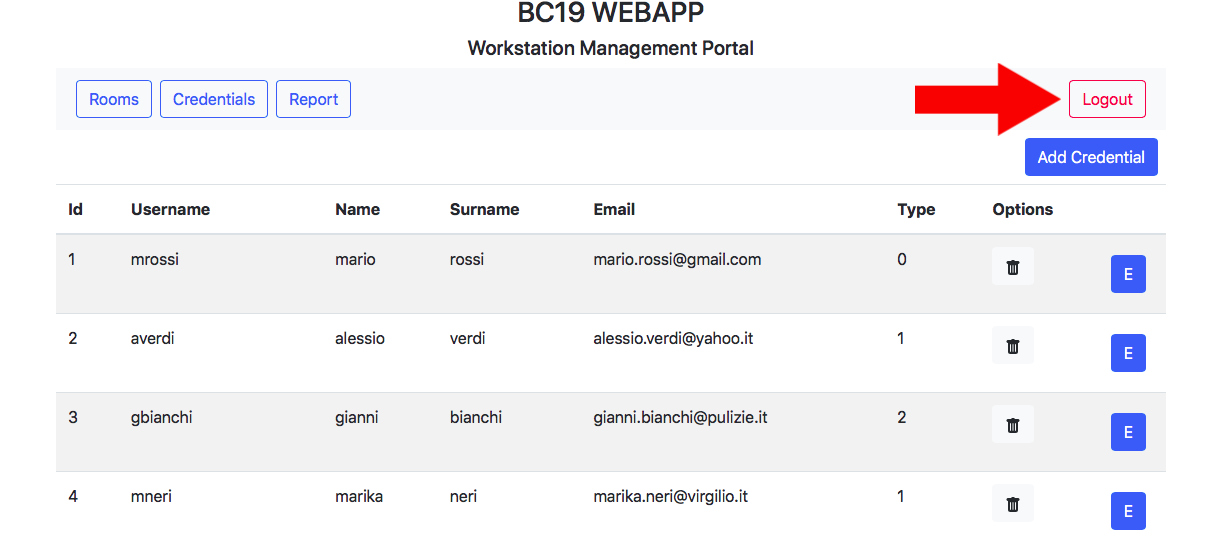
\includegraphics[width=15cm]{res/images/logout.jpg}
	\caption{Logout}
\end{figure}
L'amministratore, una volta effettuata l'autenticazione, può eseguire il logout da qualsiasi pagina della web-app. Sarà sufficiente cliccare sul pulsante in alto a destra denominato 'Logout'.

\subsubsection{Visualizzazione di una stanza}
\begin{figure}[H]
	\centering
	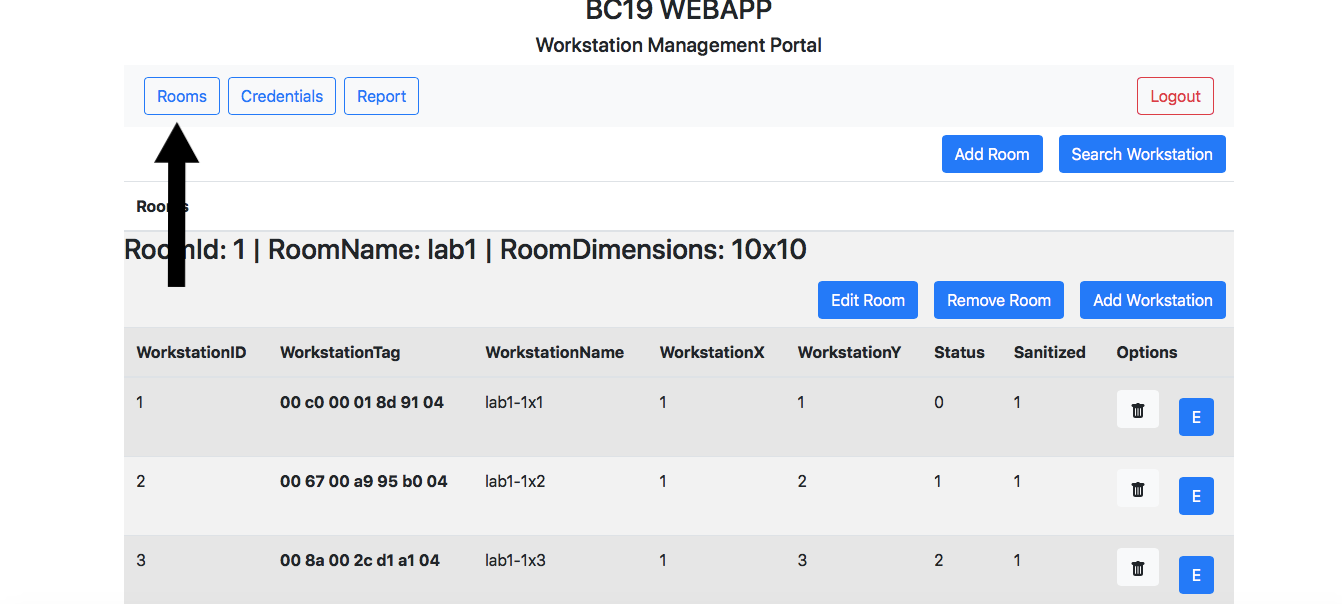
\includegraphics[width=15cm]{res/images/visStanza.png}
	\caption{Visualizzazione stanze}
\end{figure}
Per poter visualizzare le stanze, l'amministratore deve premere sul bottone 'Stanze'.
Dopo aver premuto sul bottone, per ogni stanza l'amministratore visualizza:
\begin{enumerate}
	\item identificativo della stanza;
	\item nome della stanza;
	\item dimensioni della stanza;
	\item il numero di occupanti della stanza;
	\item eventuali date in cui la stanza non è accessibile.
\end{enumerate}
Per ogni postazione all'interno di una stanza, dopo aver premuto sulla postazione di interesse, l'amministratore visualizza:
\begin{enumerate}
	\item identificativo della postazione;
	\item identificativo del tag;
	\item il nome della postazione;
	\item l'ascissa della postazione nella stanza;
	\item l'ordinata della postazione nella stanza;
	\item lo stato della postazione;
	\item lo stato dell'igienizzazione;
	\item opzione per eliminare la postazione;
	\item opzione per modificare la postazione.
	
\end{enumerate}

\subsubsection{Aggiunta di una stanza}
Per poter aggiungere una stanza, l'amministratore deve premere sul bottone 'Crea una stanza'.
\begin{figure}[H]
	\centering
	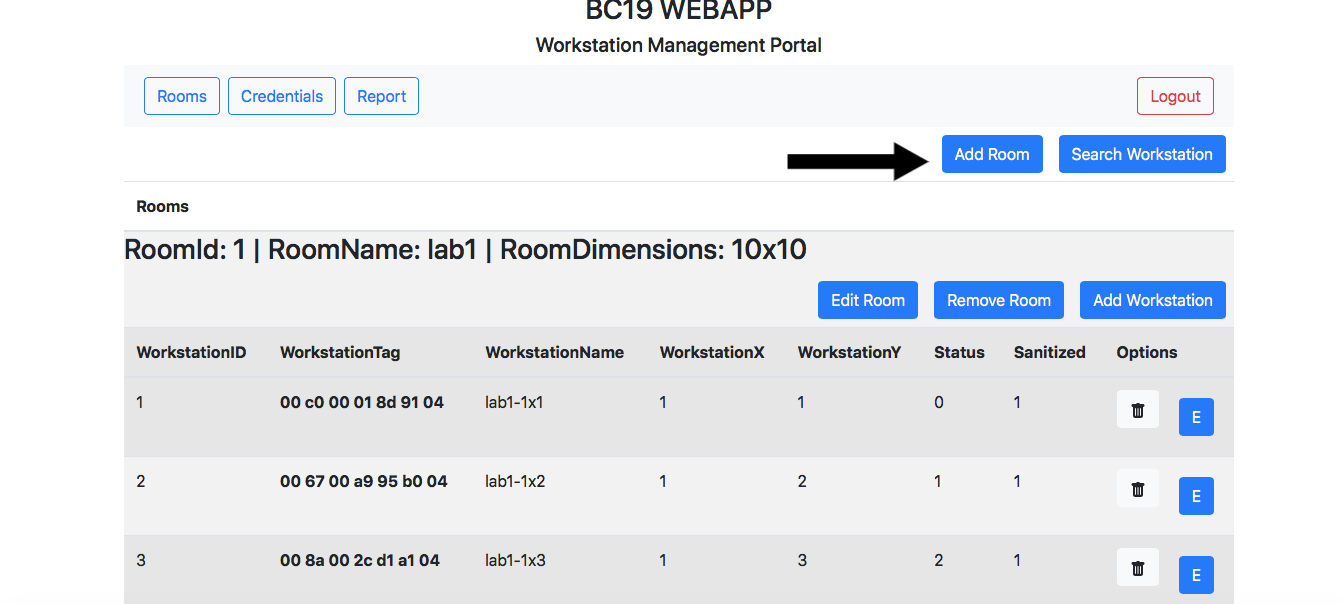
\includegraphics[width=15cm]{res/images/bottoneAddRoom.png}
	\caption{Visualizzazione bottoni}
\end{figure}
Una volta premuto sul bottone, comparirà un popup che l'amministratore dovrà compilare inserendo:
\begin{enumerate}
	\item il nome della stanza;
	\item la dimensione X;
	\item la dimensione Y.
\end{enumerate}
\begin{figure}[H]
	\centering
	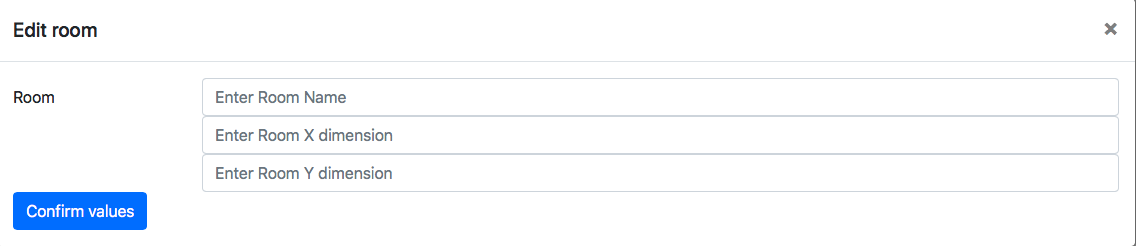
\includegraphics[width=15cm]{res/images/aggiungiStanza1.png}
	\caption{Visualizzazione popup aggiunta stanza}
\end{figure}

\subsubsection{Ricerca di una stanza}
Per poter ricercare una determinata stanza, l'amministratore deve premere sul bottone 'Cerca una stanza'.
\begin{figure}[H]
	\centering
	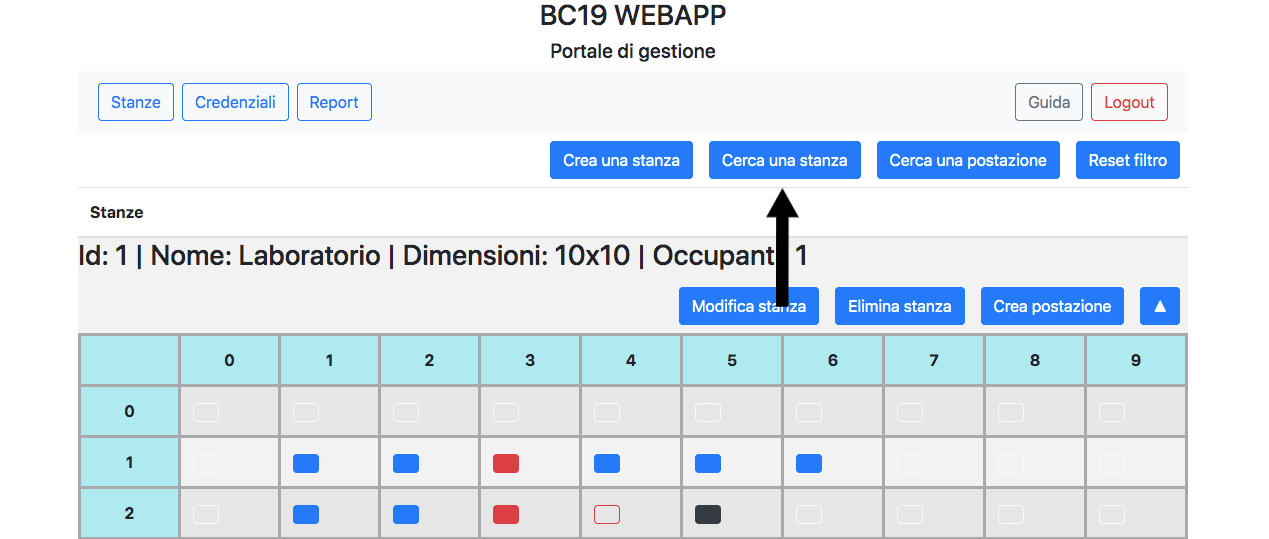
\includegraphics[width=15cm]{res/images/bottoneSearchRoom.png}
	\caption{Visualizzazione bottoni}
\end{figure}
Una volta premuto sul bottone, comparirà un popup che l'amministratore dovrà compilare inserendo il nome della stanza.
\begin{figure}[H]
	\centering
	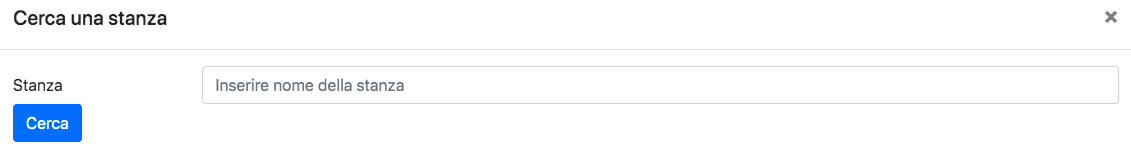
\includegraphics[width=15cm]{res/images/searchRoom.png}
	\caption{Visualizzazione popup ricerca stanza}
\end{figure}

\subsubsection{Ricerca di una postazione}
Per poter ricercare una determinata postazione, l'amministratore deve premere sul bottone 'Cerca una postazione'.
\begin{figure}[H]
	\centering
	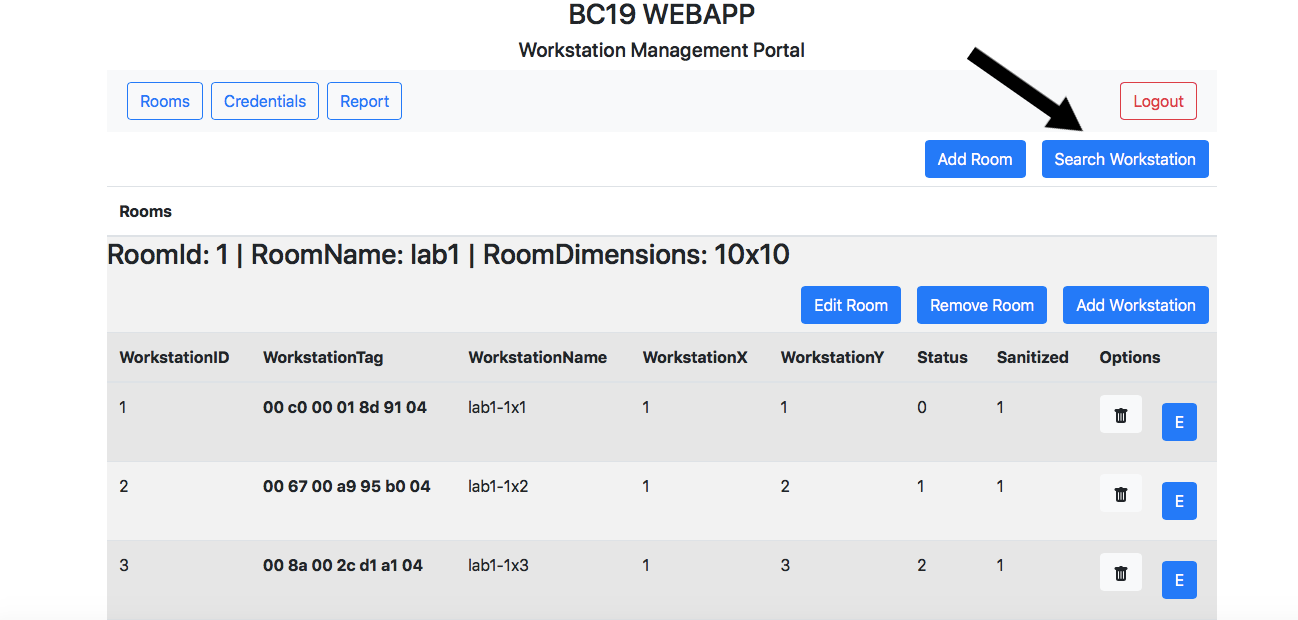
\includegraphics[width=15cm]{res/images/bottoneSearchWorkstation.png}
	\caption{Visualizzazione bottoni}
\end{figure}
Una volta premuto sul bottone, comparirà un popup che l'amministratore dovrà compilare inserendo:
l'identificativo della postazione, oppure l'username di chi la occupa.
\begin{figure}[H]
	\centering
	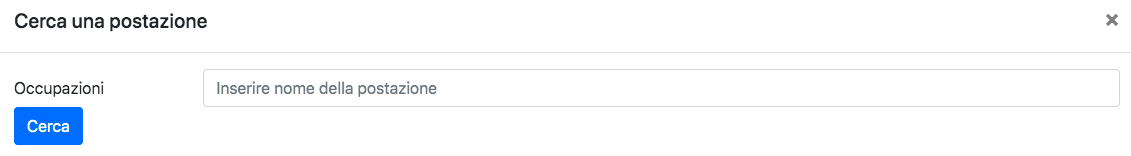
\includegraphics[width=15cm]{res/images/searchWorkstation.png}
	\caption{Visualizzazione popup ricerca postazione}
\end{figure}

\subsubsection{Reset dei filtri dopo le ricerche}
Dopo aver fatto ricerche sulla postazione e / o stanza, l'amministratore per poter tornare alla visualizzazione senza filtri per le ricerche, deve premere sul bottone 'Reset filtro'.
\begin{figure}[H]
	\centering
	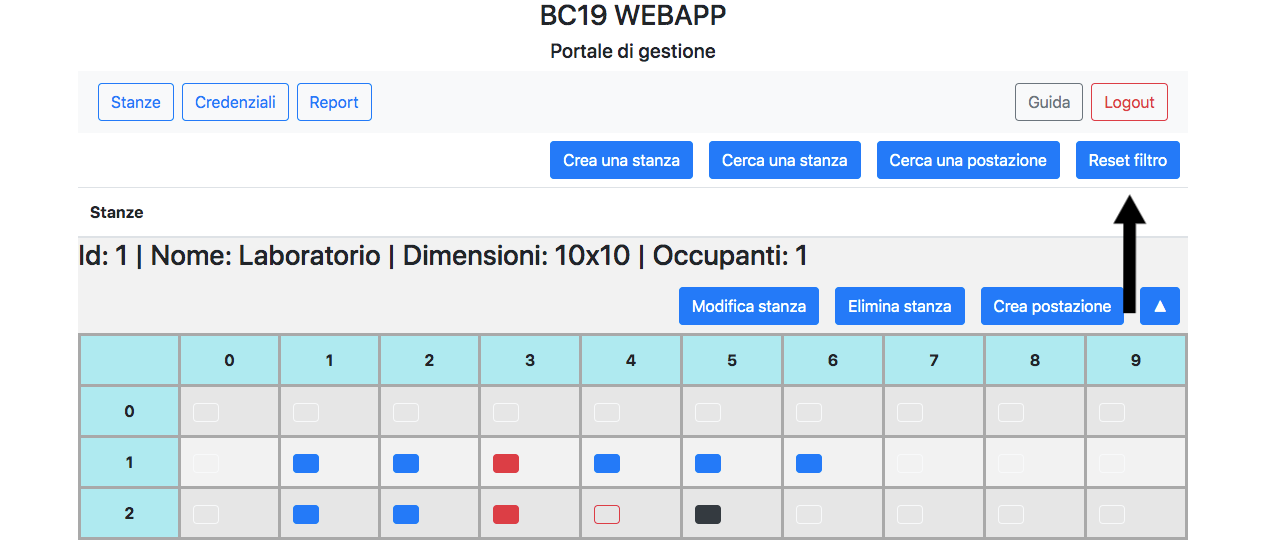
\includegraphics[width=15cm]{res/images/resetFiltri.png}
	\caption{Visualizzazione bottone}
\end{figure}

\subsubsection{Modifica di una stanza}
Per poter modificare le caratteristiche di una stanza, l'amministratore deve premere sul bottone 'Modifica stanza'.
\begin{figure}[H]
	\centering
	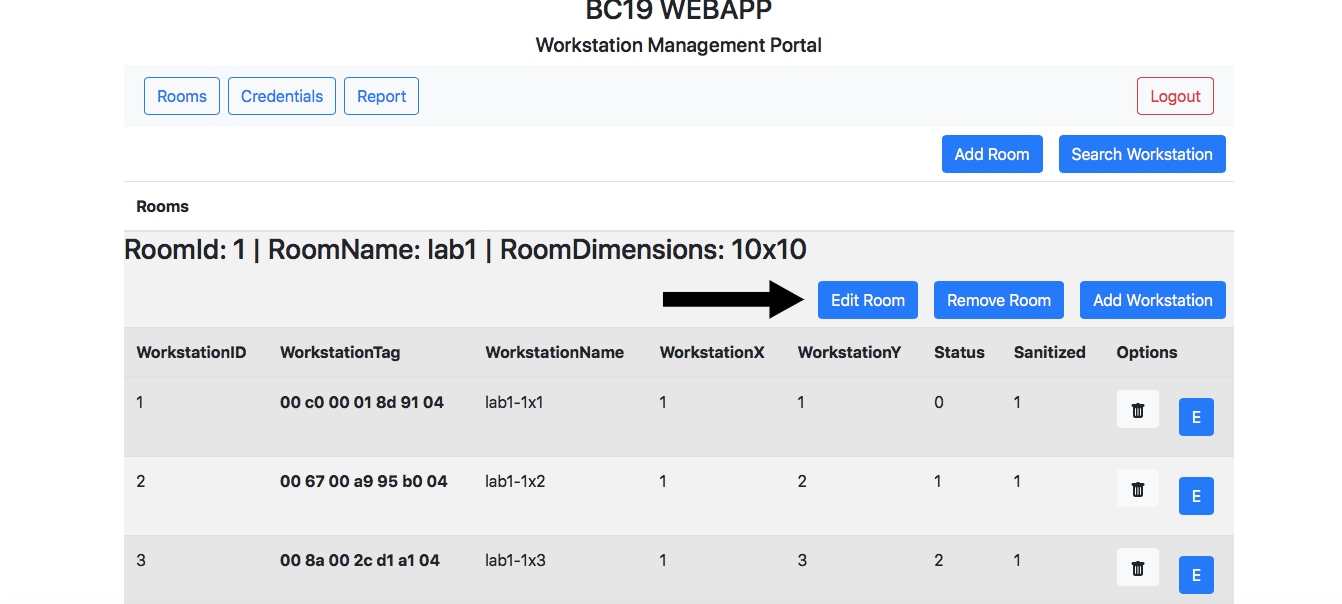
\includegraphics[width=15cm]{res/images/bottoneEditRoom.png}
	\caption{Visualizzazione bottoni}
\end{figure}
Una volta premuto sul bottone, comparirà un popup che l'amministratore dovrà compilare inserendo:
\begin{enumerate}
	\item il nome della stanza;
	\item la dimensione X;
	\item la dimensione Y.
\end{enumerate}
\begin{figure}[H]
	\centering
	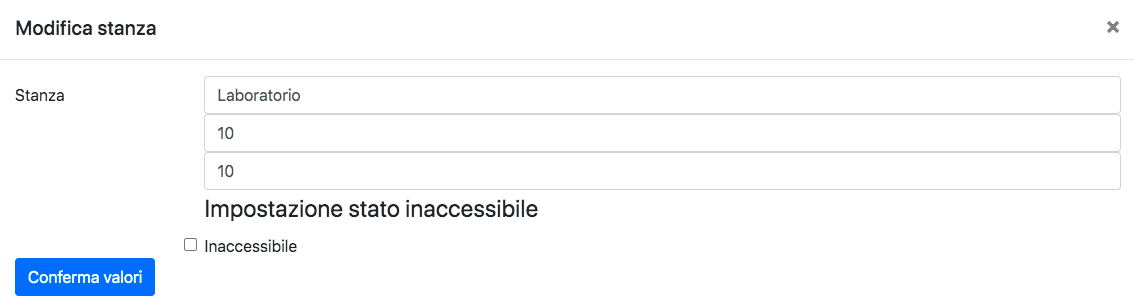
\includegraphics[width=15cm]{res/images/modificaStanza.png}
	\caption{Visualizzazione popup modifica stanza}
\end{figure}

\subsubsection{Impostazione di una stanza come inaccessibile}
Per poter modificare le caratteristiche di una stanza impostandola come inaccessibile, l'amministratore deve premere sul bottone 'Modifica Stanza'.
\begin{figure}[H]
	\centering
	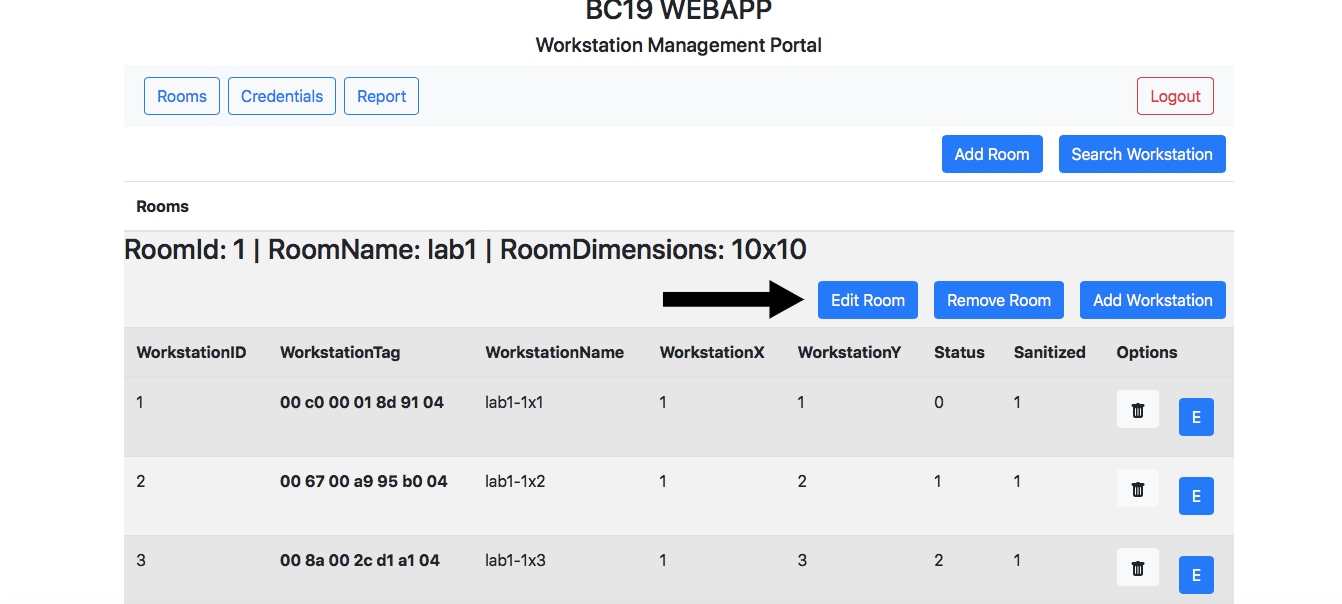
\includegraphics[width=15cm]{res/images/bottoneEditRoom.png}
	\caption{Visualizzazione bottoni}
\end{figure}
Una volta premuto sul bottone, comparirà un popup dove l'amministratore dovrà selezionare il checkbox per inserire le date in cui la stanza sarà inaccessibile, e selezionerà:
\begin{enumerate}
	\item data inizio inaccessibilità;
	\item data fine inaccessibilità.
\end{enumerate}
\begin{figure}[H]
	\centering
	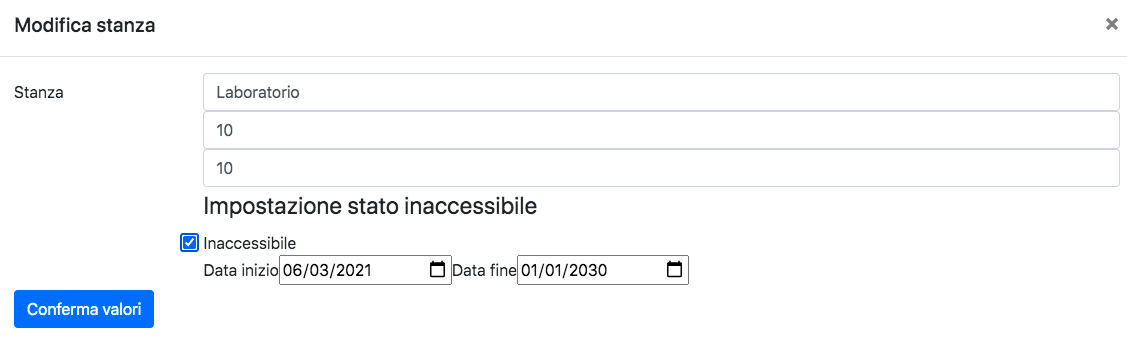
\includegraphics[width=15cm]{res/images/roomInaccessibile.png}
	\caption{Visualizzazione popup modifica stanza come inaccessibile}
\end{figure}

\subsubsection{Rimozione di una stanza}
Per poter rimuovere una stanza, l'amministratore deve premere sul bottone 'Elimina stanza'.
\begin{figure}[H]
	\centering
	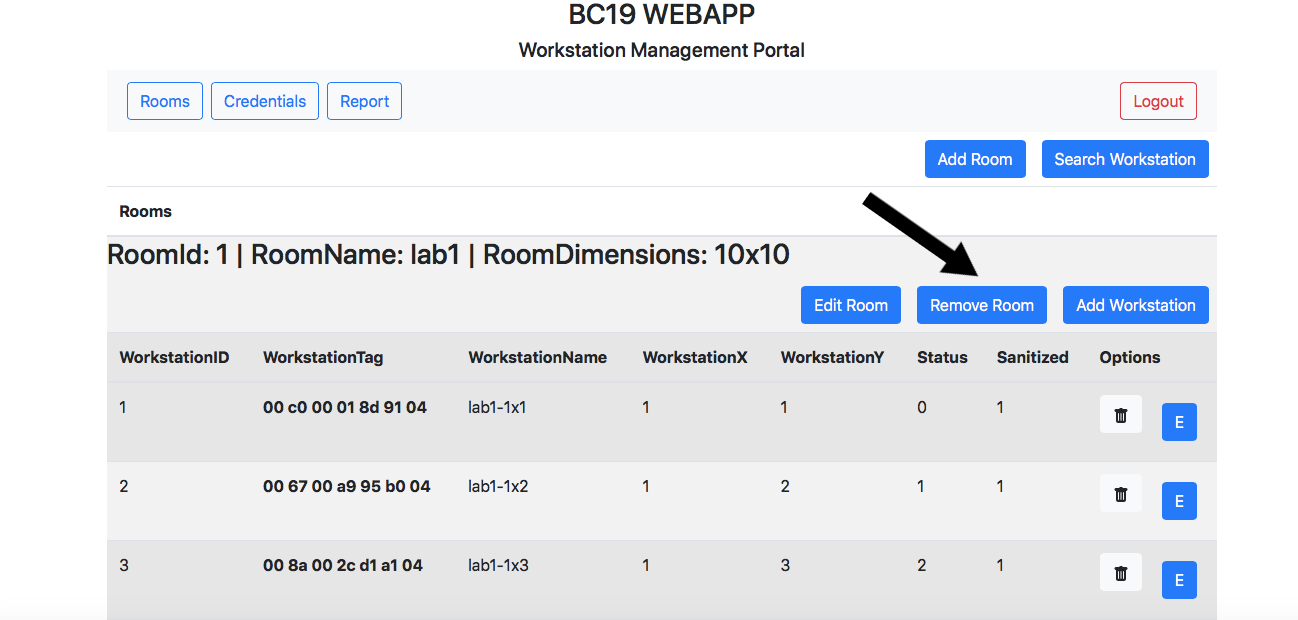
\includegraphics[width=15cm]{res/images/bottoneRemoveRoom.png}
	\caption{Visualizzazione bottoni}
\end{figure}
Una volta premuto sul bottone, comparirà un popup che chiederà all'amministratore una conferma per eliminare definitivamente la stanza.

\subsubsection{Aggiunta di una postazione all'interno di una stanza}
Per poter inserire una nuova postazione all'interno di una stanza, l'amministratore deve premere sul bottone 'Add Workstation'.
\begin{figure}[H]
	\centering
	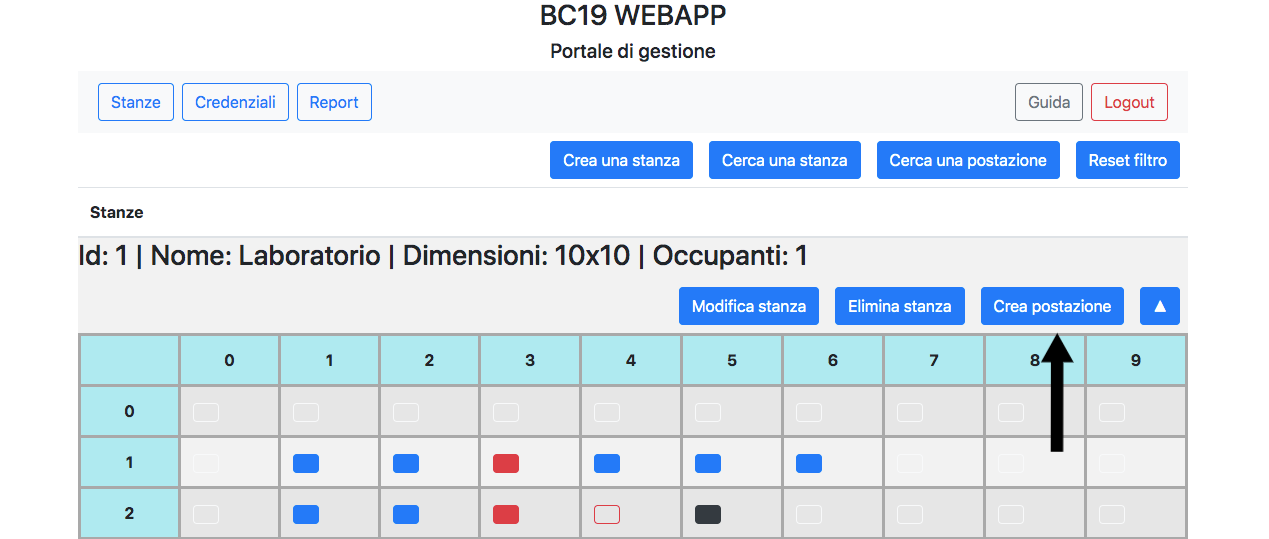
\includegraphics[width=15cm]{res/images/bottoneAddWorkstation.png}
	\caption{Visualizzazione bottoni}
\end{figure}
Una volta premuto sul bottone, comparirà un popup che l'amministratore dovrà compilare inserendo:
\begin{enumerate}
	\item il tag della postazione;
	\item il nome della postazione;
	\item la dimensione X della postazione nella stanza;
	\item la dimensione Y della postazione nella stanza.
\end{enumerate}
\begin{figure}[H]
	\centering
	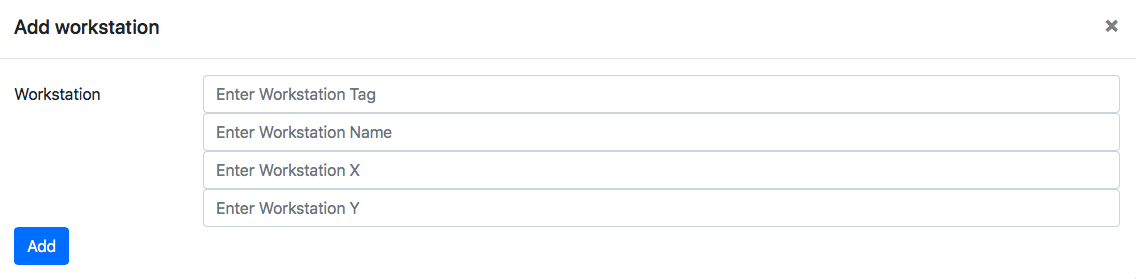
\includegraphics[width=15cm]{res/images/addWorkstation.png}
	\caption{Visualizzazione popup inserimento postazione dentro a una stanza}
\end{figure}

\subsubsection{Eliminazione di una postazione all'interno di una stanza}
Per poter eliminare una postazione all'interno di una stanza, l'amministratore deve premere sul bottone dove è raffigurato un cestino.
\begin{figure}[H]
	\centering
	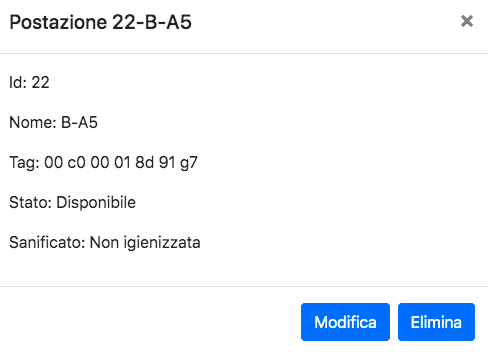
\includegraphics[width=15cm]{res/images/bottoneCestinoWorkstation.png}
	\caption{Visualizzazione bottoni}
\end{figure}
Una volta premuto sul bottone, comparirà un popup che chiederà all' amministratore una conferma per eliminare definitivamente la postazione dentro alla stanza.

\subsubsection{Modifica di una postazione all'interno di una stanza}
Per poter modificare le caratteristiche di una postazione all'interno di una stanza, l'amministratore deve premere sul bottone 'E' di colore blu.
\begin{figure}[H]
	\centering
	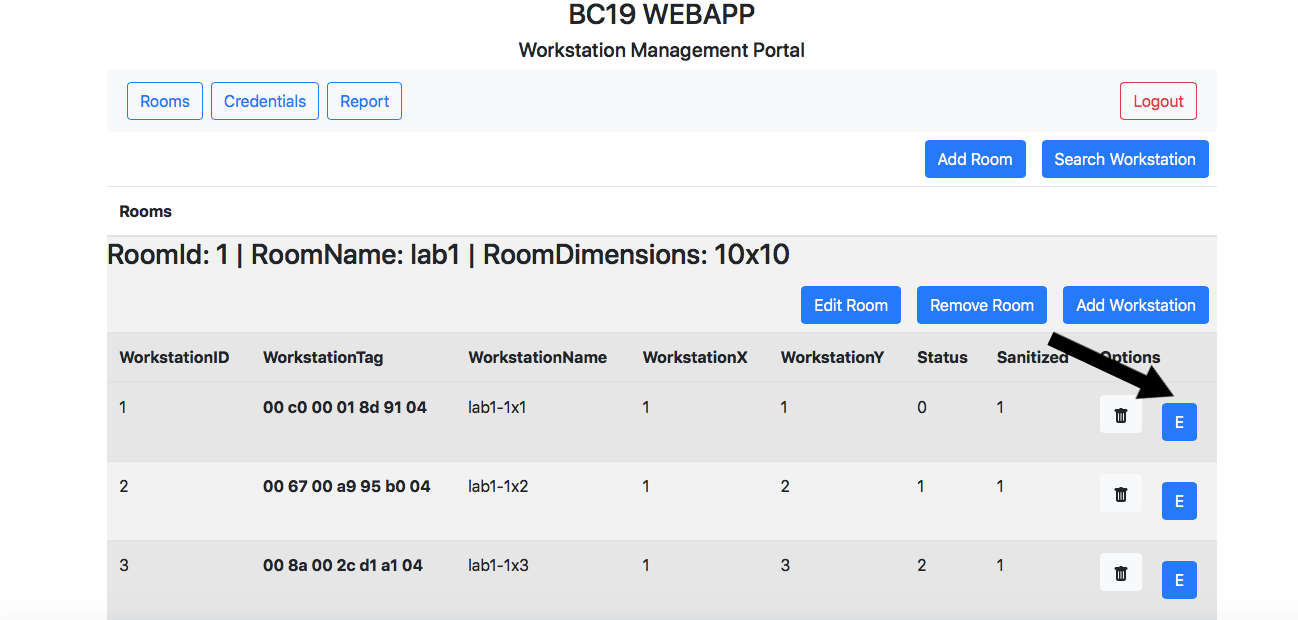
\includegraphics[width=15cm]{res/images/bottoneEditWorkstation.png}
	\caption{Visualizzazione bottoni}
\end{figure}
Una volta premuto sul bottone, comparirà un popup che l'amministratore dovrà compilare inserendo:
\begin{enumerate}
	\item il tag della postazione;
	\item il nome della postazione;
	\item la dimensione X della postazione nella stanza;
	\item la dimensione Y della postazione nella stanza.
\end{enumerate}
\begin{figure}[H]
	\centering
	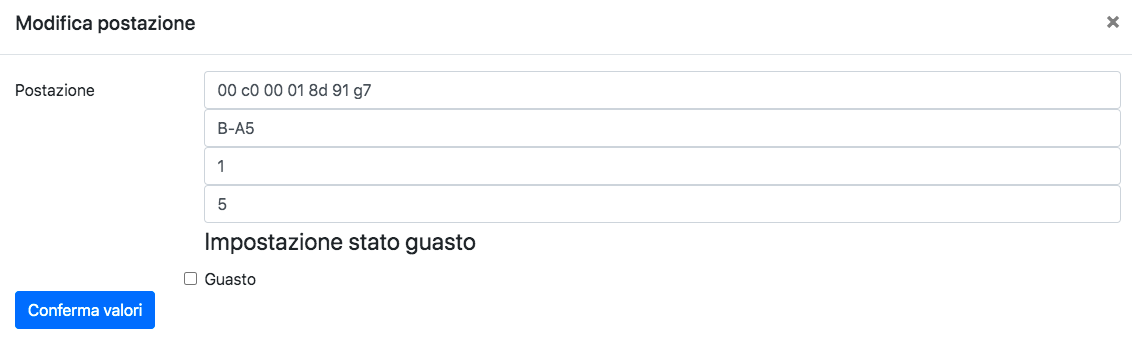
\includegraphics[width=15cm]{res/images/editWorkstation.png}
	\caption{Visualizzazione popup modifica postazione all'interno di una stanza}
\end{figure}

\subsubsection{Visualizzazione delle credenziali}
\begin{figure}[H]
	\centering
	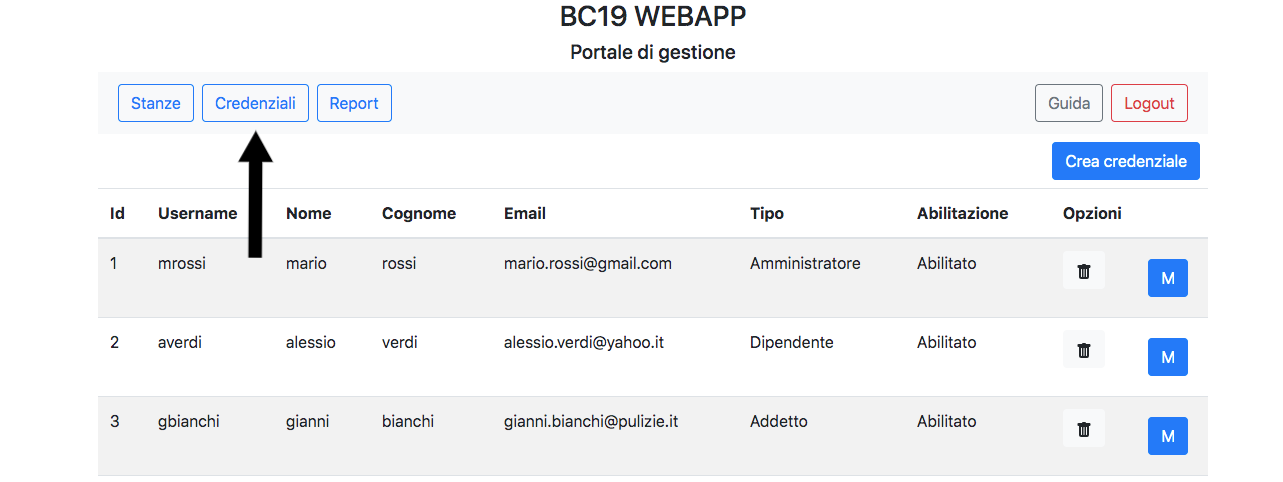
\includegraphics[width=15cm]{res/images/credential.png}
	\caption{Visualizzazione credenziali}
\end{figure}
L’amministratore può visualizzare la lista delle credenziali di ogni utente. Questo sarà permesso da ogni pagina cliccando sul pulsante Credenziali.
La lista di credenziali è composta dai seguenti campi:
\begin{enumerate}
	\item Id;
	\item Username;
	\item Nome;
	\item Cognome;
	\item Email;
	\item Tipo;
	\item Abilitazione;
	\item Opzioni.
\end{enumerate}
Titpo indica il tipo di utente, Opzioni presenta due pulsanti per eliminare o modificare le credenziali e Abilitazione indica se le credenziali di quell'utente sono abilitate oppure no.

\subsubsection{Aggiunta di nuove credenziali}
Per poter aggiungere nuove credenziali, l'amministratore deve premere sul bottone 'Crea credenziale' di colore blu.
\begin{figure}[H]
	\centering
	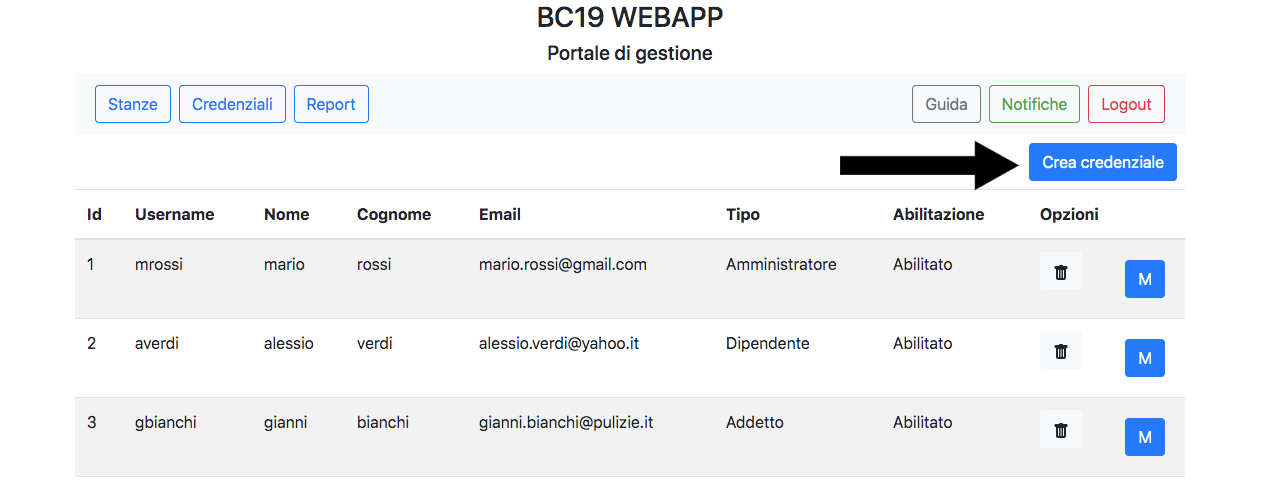
\includegraphics[width=15cm]{res/images/addCredential.jpg}
	\caption{Bottone di aggiunta credenziali}
\end{figure}
Una volta premuto sul bottone, comparirà un popup che l'amministratore dovrà compilare inserendo:
\begin{enumerate}
	\item il nome dell'utente;
	\item il cognome dell'utente;
	\item l'username;
	\item l'email;
	\item il tipo di utente;
	\item la password.
\end{enumerate}
\begin{figure}[H]
	\centering
	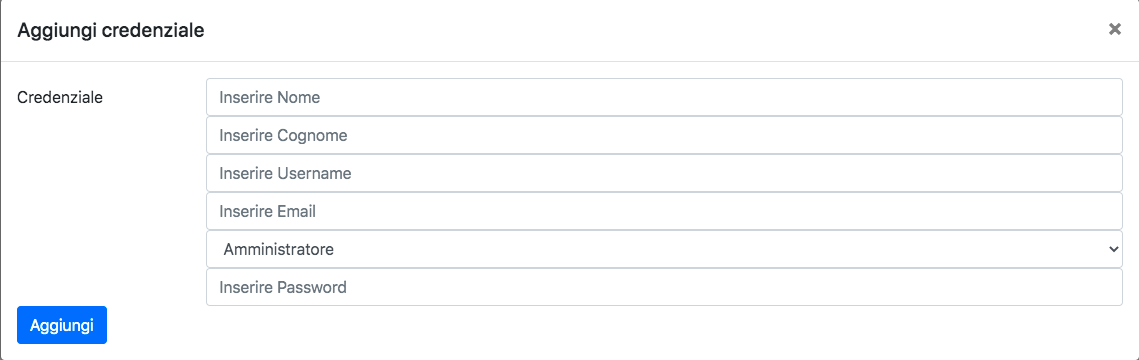
\includegraphics[width=15cm]{res/images/addc.jpg}
	\caption{Visualizzazione popup di inserimento credenziali}
\end{figure}


\subsubsection{Eliminazione delle credenziali}
Per poter eliminare le credenziali di un utente, l'amministratore deve premere sul bottone che raffigura il cestino.
\begin{figure}[H]
	\centering
	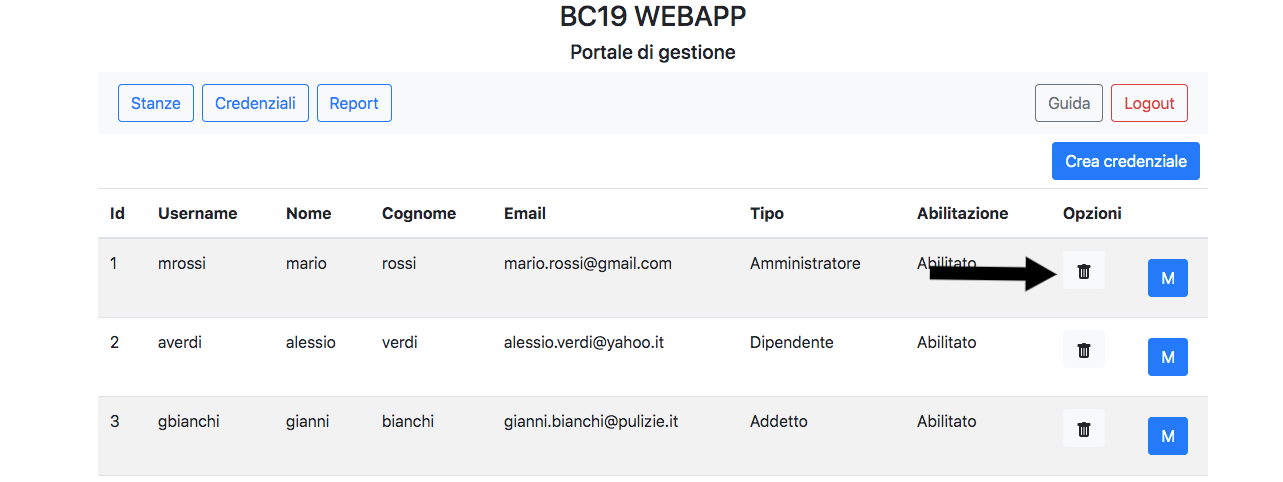
\includegraphics[width=15cm]{res/images/optionDelete.jpg}
	\caption{Bottone di cancellazione credenziali}
\end{figure}

\subsubsection{Modifica delle credenziali}
Per poter modificare le credenziali di un utente, l'amministratore deve premere sul bottone 'M' di colore blu.
\begin{figure}[H]
	\centering
	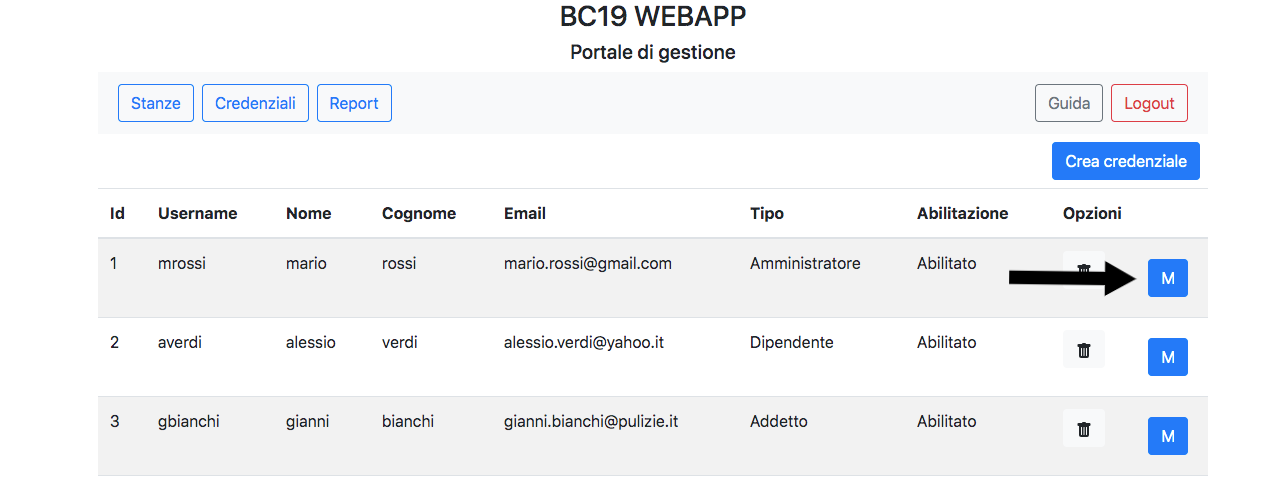
\includegraphics[width=15cm]{res/images/optionEdit.jpg}
	\caption{Bottone di modifica credenziali}
\end{figure}
Una volta premuto sul bottone, comparirà un popup che l'amministratore dovrà compilare inserendo:
\begin{enumerate}
	\item il nome dell'utente;
	\item il cognome dell'utente;
	\item l'username;
	\item l'email;
	\item il tipo di utente;
	\item la password;
	\item abilitato / non abilitato.
\end{enumerate}
\begin{figure}[H]
	\centering
	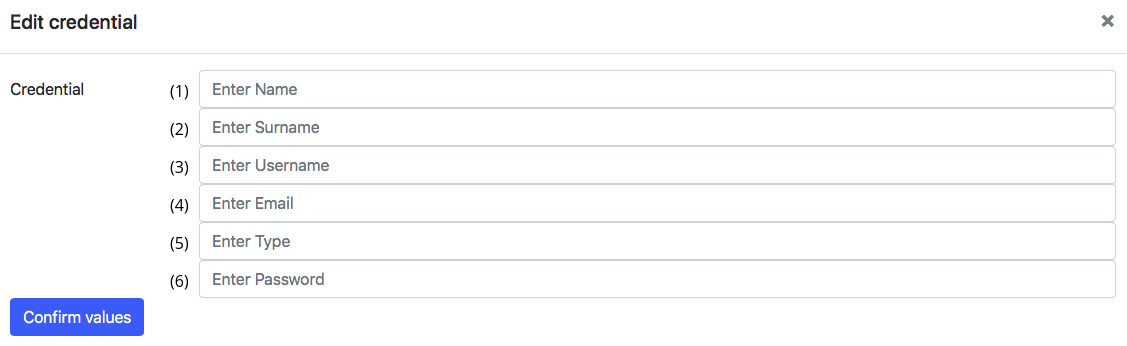
\includegraphics[width=15cm]{res/images/editc.jpg}
	\caption{Visualizzazione popup modifica credenziali}
\end{figure}

\subsubsection{Visualizzazione della Guida}
Per poter visualizza il Manuale Utente dell'applicazione, l'amministratore deve premere sul bottone 'Guida'. In seguito in una nuova pagina del browser, verrà aperta in formato PDF la Guida (Manuale Utente) dell'applicazione.
\begin{figure}[H]
	\centering
	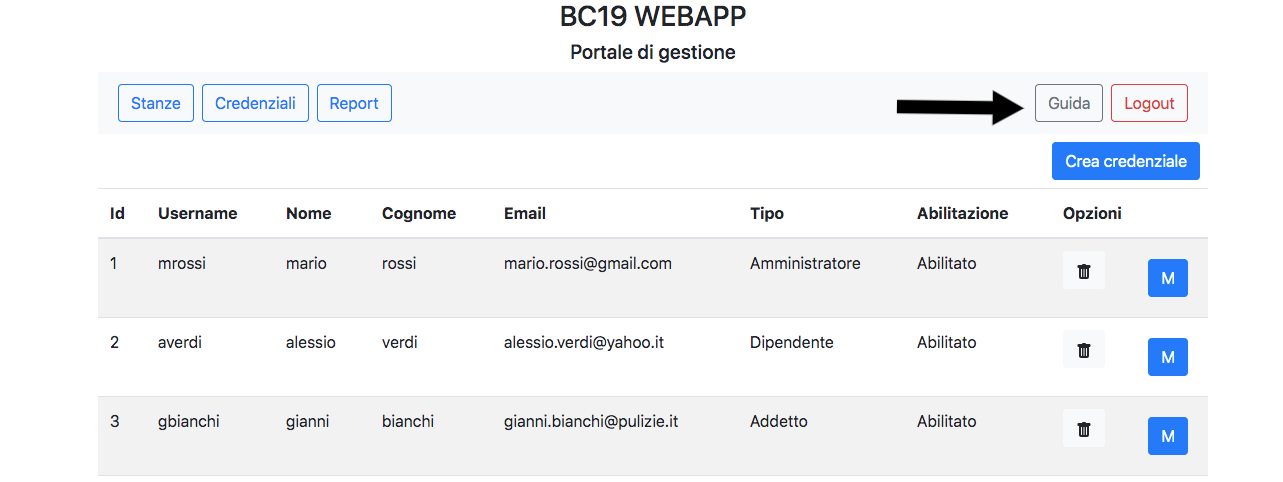
\includegraphics[width=15cm]{res/images/guida.jpg}
	\caption{Visualizzazione Guida}
\end{figure}
